\documentclass[dvipsnames, usenames]{beamer}

\usetheme{cleancode}
\usepackage[T1]{fontenc}
\usepackage[ansinew]{inputenc}
\usepackage[USenglish]{babel}
\usepackage{amsmath}
\usepackage{mathtools}
\usepackage{stmaryrd}
\usepackage{graphicx}
\usepackage{lmodern}
%\usepackage{tcolorbox}

\usepackage[round, authoryear]{natbib}
\usepackage{subcaption}
\usepackage[export]{adjustbox}

% Graph Picture Packages
\usepackage{tikz}
\usetikzlibrary{positioning}
\usetikzlibrary{calc}

\usepackage{amsthm, amssymb, amsfonts, amsmath, xcolor}
\def\boxitem#1{\setbox0=\vbox{#1}{\centering\makebox[0pt]{%
  \fboxrule=2pt\color{red}\fbox{\hspace{\leftmargini}\color{black}\box0}}\par}}


\usepackage{algorithm,algorithmicx,algpseudocode}
\algnewcommand\algorithmicinput{\textbf{Input:}}
\algnewcommand\INPUT{\item[\algorithmicinput]}
\algnewcommand\algorithmicoutput{\textbf{Output:}}
\algnewcommand\OUTPUT{\item[\algorithmicoutput]}
\algnewcommand\algorithmicidea{\textbf{Idea:}}
\algnewcommand\IDEA{\item[\algorithmicidea]}
\algnewcommand\algorithmicinit{\textbf{Initialize:}}
\algnewcommand\INIT{\item[\algorithmicinit]}

\algnewcommand\algorithmicforeach{\textbf{for each}}
\algdef{S}[FOR]{ForEach}[1]{\algorithmicforeach\ #1\ \algorithmicdo}


\newcommand\Wider[2][3em]{%
\makebox[\linewidth][c]{%
  \begin{minipage}{\dimexpr\textwidth+#1\relax}
  \raggedright#2
  \end{minipage}%
  }%
}

\usepackage{bibentry, bibentry}

% Generates new title page at beginning of each section
\AtBeginSection[]{
  \begin{frame}
  \vfill
  \centering
  \begin{beamercolorbox}[sep=8pt,center,shadow=true,rounded=true]{title}
    \usebeamerfont{title}\insertsectionhead\par%
  \end{beamercolorbox}
  \vfill
  \end{frame}
}
\setbeamertemplate{navigation symbols}{}


\DeclareMathOperator*{\plim}{plim}

\setbeamertemplate{footline}[frame number]
\setbeamertemplate{theorems}[numbered]

\newcommand{\R}{\mathbb{R}}
\newcommand{\N}{\ensuremath{\mathcal{N}}}

\pgfdeclareimage[width=0.7\paperwidth]{mybackground}{../figures/report/datasets}
%
%\setbeamertemplate{title page}{
%
%        \begin{picture}(0,0)
%
%            \put(-30,-100){%
%                \pgfuseimage{mybackground}
%            }
%
%            \put(0,-110.7){%
%                \begin{minipage}[b][45mm][t]{226mm}
%                    \usebeamerfont{title}{\inserttitle\par}
%                    	\usebeamerfont{author}{\insertauthor\par}
%                \end{minipage}
%            }
%
%            \end{picture}
%
%    }

\usepackage{enumitem,amssymb}
\newlist{todolist}{itemize}{2}
\setlist[todolist]{label=$\square$}
\usepackage{pifont}
\newcommand{\cmark}{\ding{51}}%
\newcommand{\xmark}{\ding{55}}%
\newcommand{\done}{\rlap{$\square$}{\raisebox{2pt}{\large\hspace{1pt}\cmark}}%
\hspace{-2.5pt}}
\newcommand{\wontfix}{\rlap{$\square$}{\large\hspace{1pt}\xmark}}


\usepackage[customcolors]{hf-tikz}

\hfsetfillcolor{white}
\hfsetbordercolor{red}
\usepackage{tcolorbox}

\begin{document}

%------------------------------------------------------------------------------%
% Setup TikzStyle

\tikzstyle{block} = [rectangle, draw, 
    text width=5em, text centered, rounded corners, minimum height=1.5em]
    
\tikzstyle{line} = [draw, -latex]

\title{Biologically Plausible Deep Learning: \\ A Critical Review of \citet{guerguiev2017} \thanks{Guerguiev, J., Lillicrap, T. P., \& Richards, B. A. (2017). Towards deep learning with segregated dendrites. ELife, 6, e22901.}}
\subtitle{}

\author{\texorpdfstring{Robert Tjarko Lange\thanks{Code: \url{github.com/RobertTLange/Bio-Plausible-DeepLearning}}
						\newline\url{rtl17@ic.ac.uk}
						\newline\url{www.rob-lange.com}
	}
	{Author}}


\institute{Einstein Center for Neurosciences Berlin}
\date{\today}


%------------------------------------------------------------------------------%

\begin{frame}[noframenumbering]

\titlepage
%\begin{picture}(0,0)
%\put(+25,+0){\pgfuseimage{mybackground}}
%\end{picture}
\end{frame}

%------------------------------------------------------------------------------%
\begin{frame}{Biologically Implausible Backpropagation}

\begin{itemize}
	\item[$\rightarrow$] MLP: $h_l \coloneqq f(h_{l-1}; \theta_l) = \sigma_l (W_l h_{l-1} + b_l), \ l=1,\dots, L$
\end{itemize}
\pause
\centering
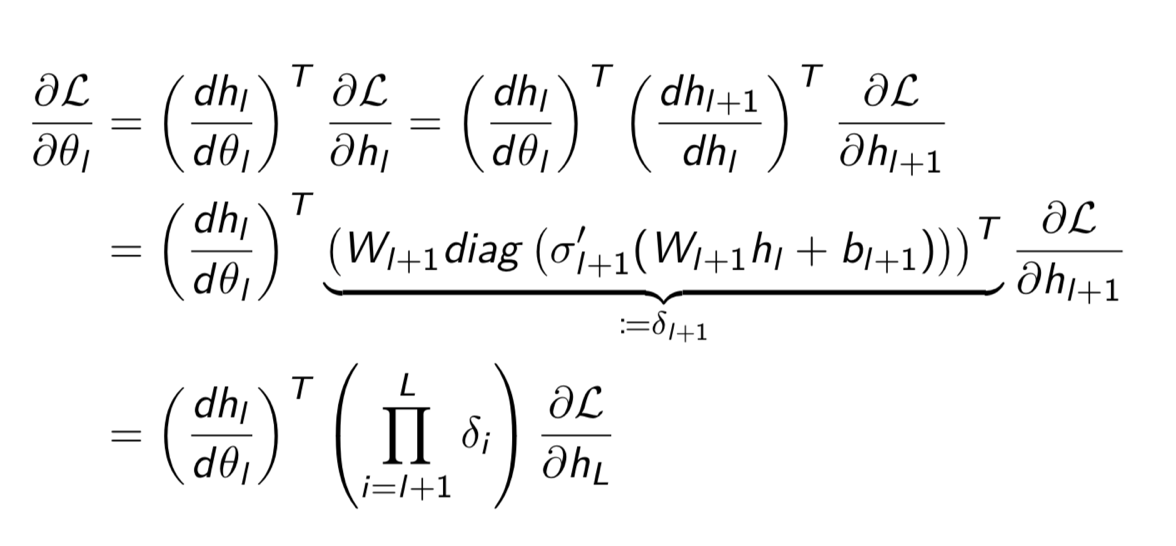
\includegraphics[width=1.1\textwidth]{../figures/report/backprop_1}

\end{frame}

%------------------------------------------------------------------------------%
\begin{frame}[noframenumbering]{Biologically Implausible Backpropagation}

\begin{itemize}
	\item[$\rightarrow$] MLP: $h_l \coloneqq f(h_{l-1}; \theta_l) = \sigma_l (W_l h_{l-1} + b_l), \ l=1,\dots, L$
\end{itemize}

\centering
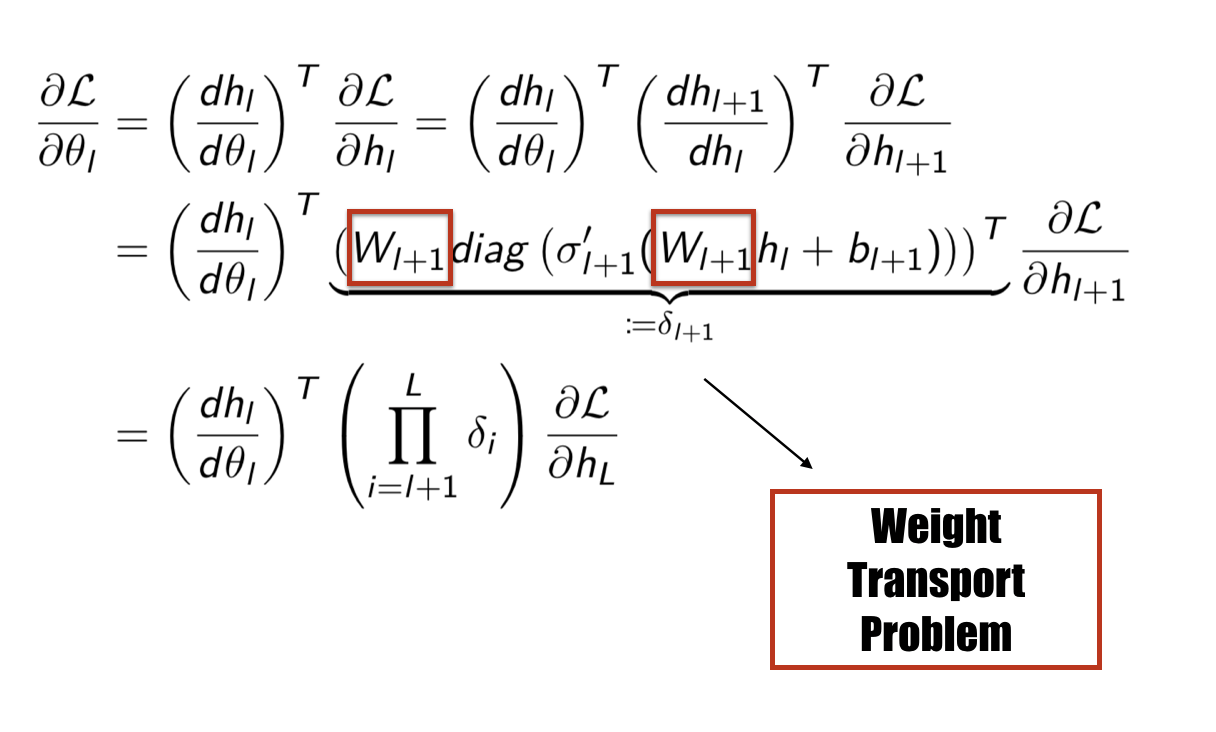
\includegraphics[width=1.1\textwidth]{../figures/report/backprop_2}

\end{frame}


%------------------------------------------------------------------------------%
\begin{frame}[noframenumbering]{Biologically Implausible Backpropagation}

\begin{itemize}
	\item[$\rightarrow$] MLP: $h_l \coloneqq f(h_{l-1}; \theta_l) = \sigma_l (W_l h_{l-1} + b_l), \ l=1,\dots, L$
\end{itemize}

\centering
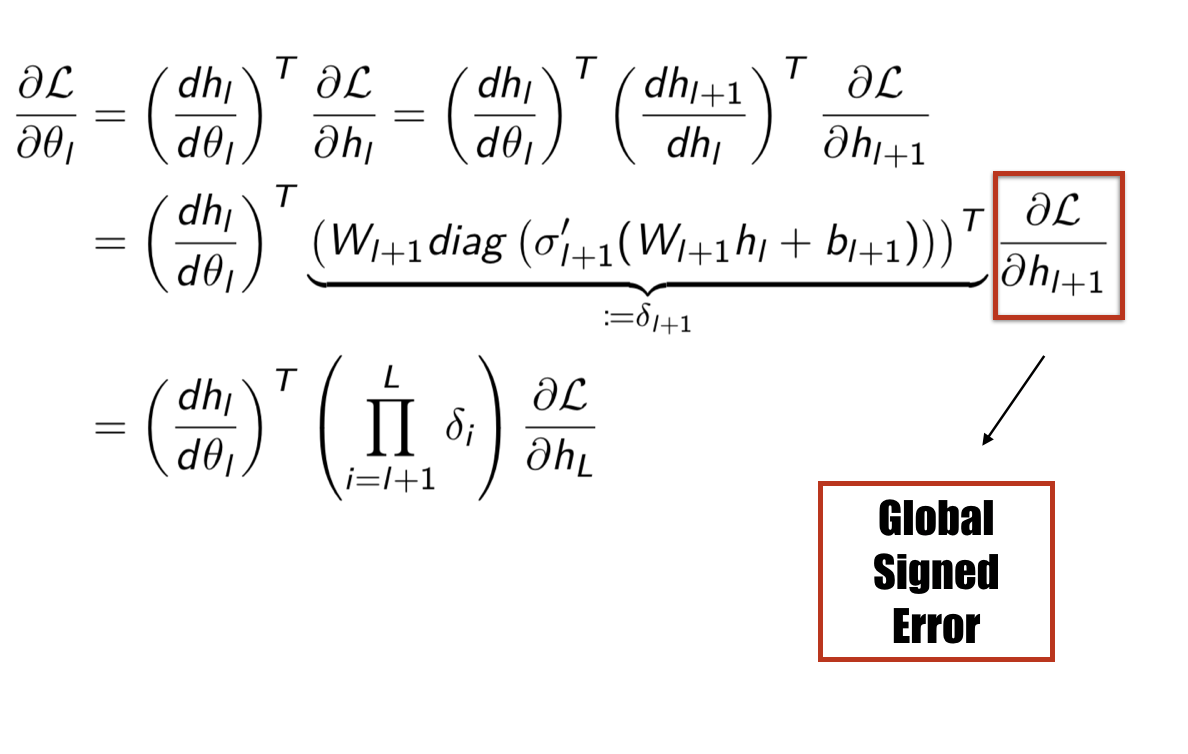
\includegraphics[width=1.1\textwidth]{../figures/report/backprop_3}

\end{frame}


%------------------------------------------------------------------------------%
\begin{frame}{A Solution - Electrical Segregation of $\downarrow$ and $\uparrow$ Info}

\centering 
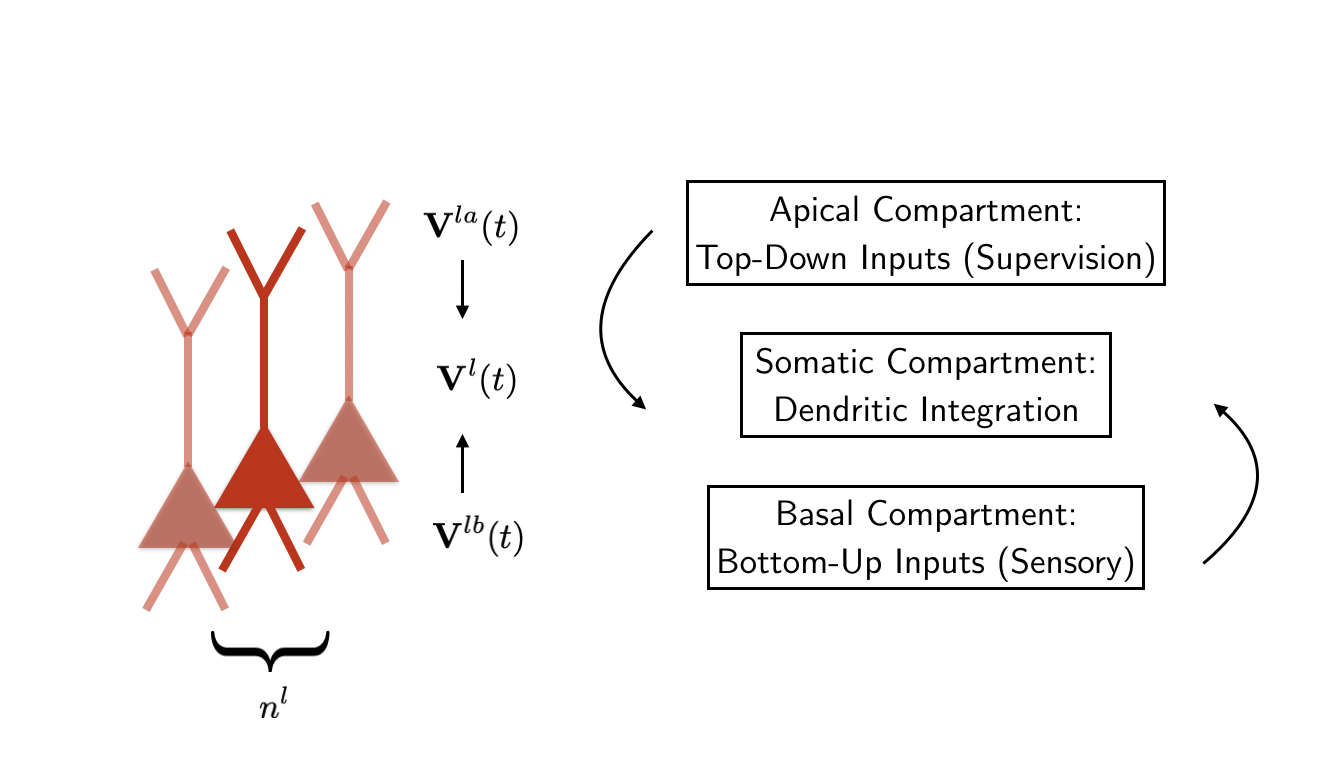
\includegraphics[width=1.1\textwidth]{../figures/report/comp_sol_1}
\end{frame}

%------------------------------------------------------------------------------%
\begin{frame}[noframenumbering]{A Solution - Electrical Segregation of $\downarrow$ and $\uparrow$ Info}

\centering 
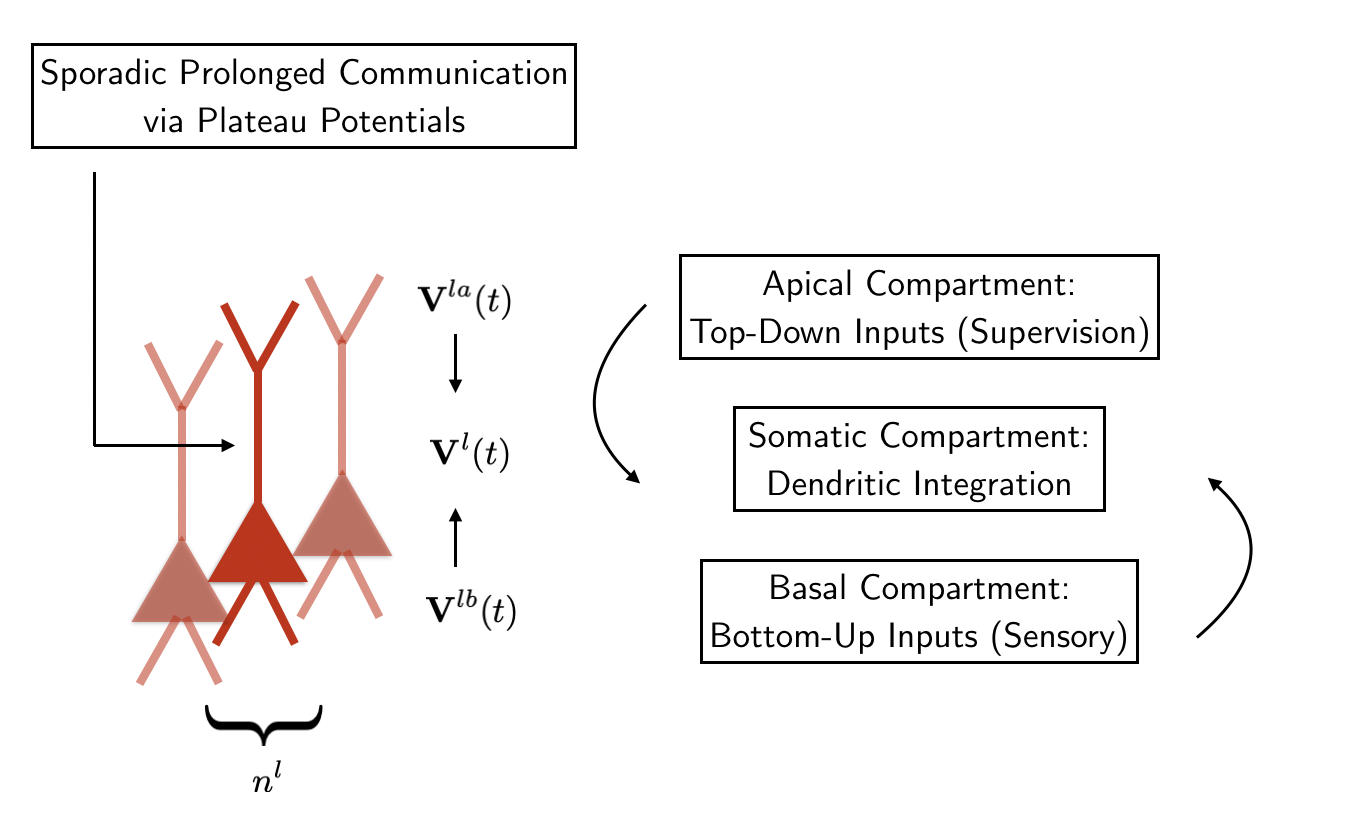
\includegraphics[width=1.1\textwidth]{../figures/report/comp_sol_2}
\end{frame}
%------------------------------------------------------------------------------%
\begin{frame}[noframenumbering]{A Solution - Electrical Segregation of $\downarrow$ and $\uparrow$ Info}

\centering 
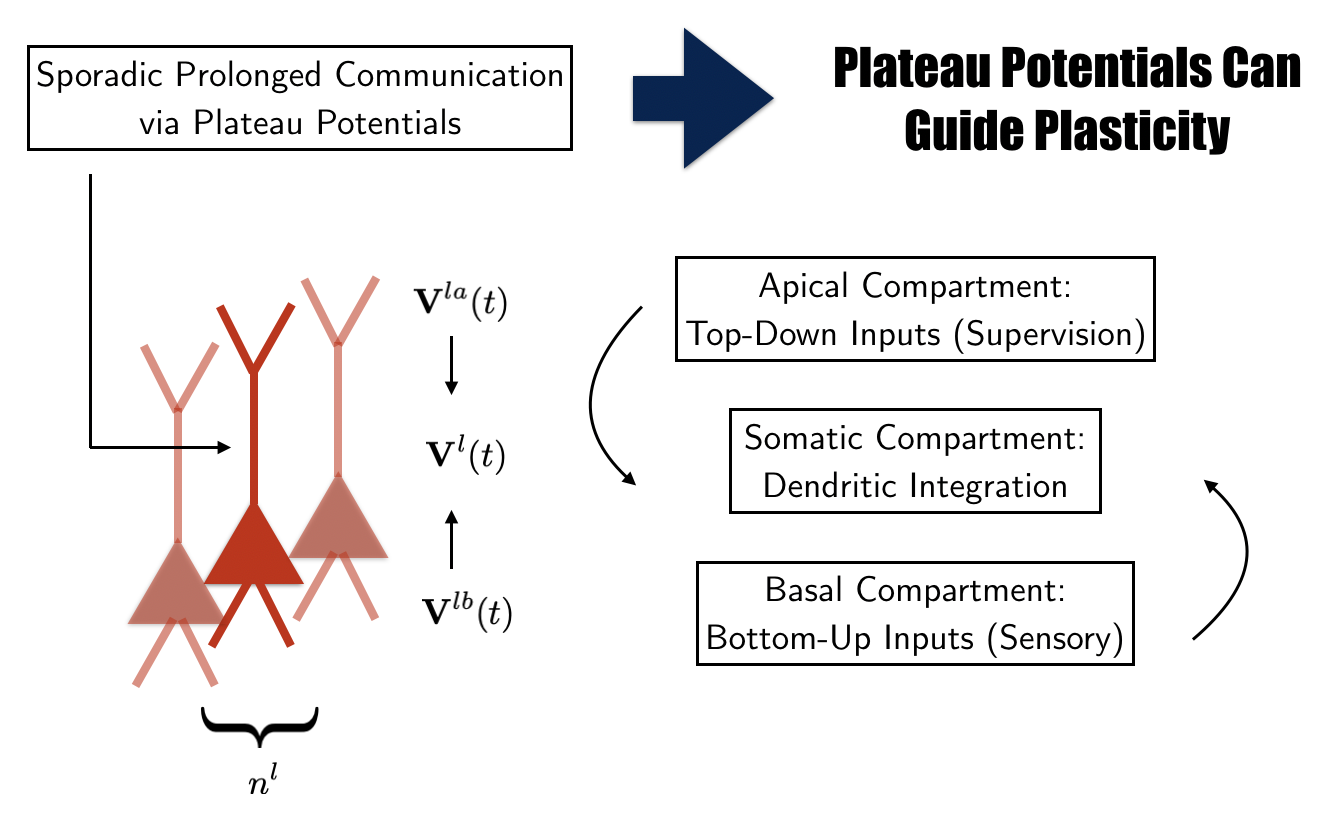
\includegraphics[width=1.1\textwidth]{../figures/report/comp_sol_3}
\end{frame}

%------------------------------------------------------------------------------%
\begin{frame}{\citet{guerguiev2017} - Hidden Layer Structure}

\centering 
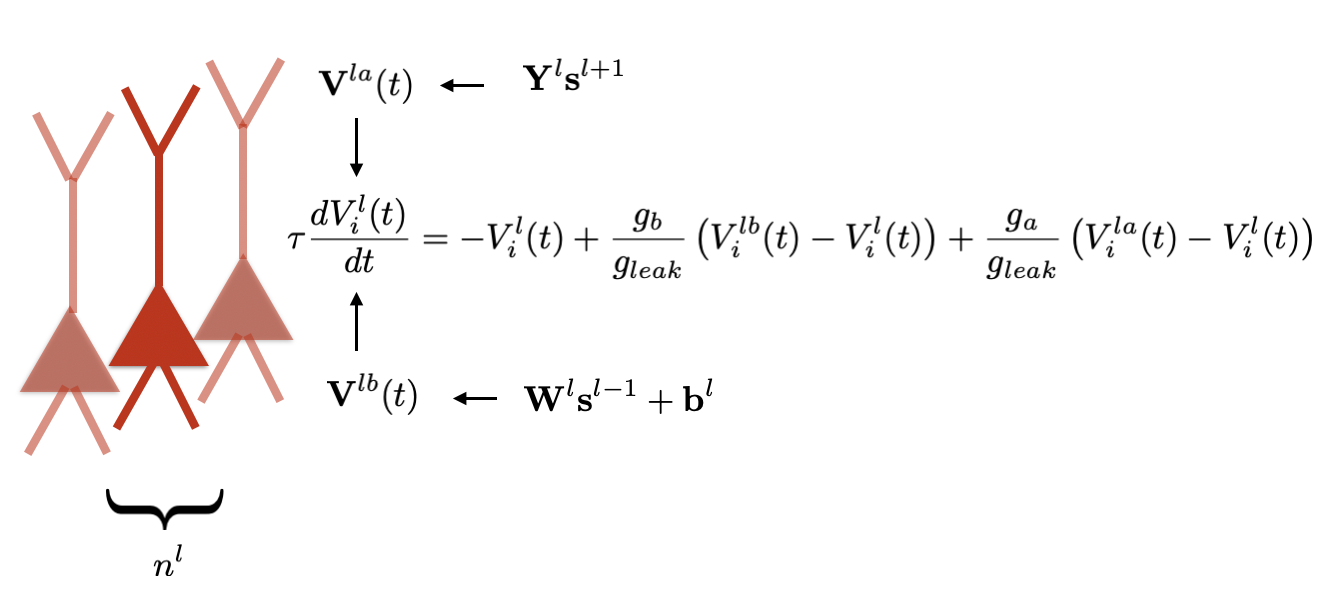
\includegraphics[width=1.1\textwidth]{../figures/report/hidden_1}
\end{frame}

%------------------------------------------------------------------------------%
\begin{frame}[noframenumbering]{\citet{guerguiev2017} - Hidden Layer Structure}

\centering 
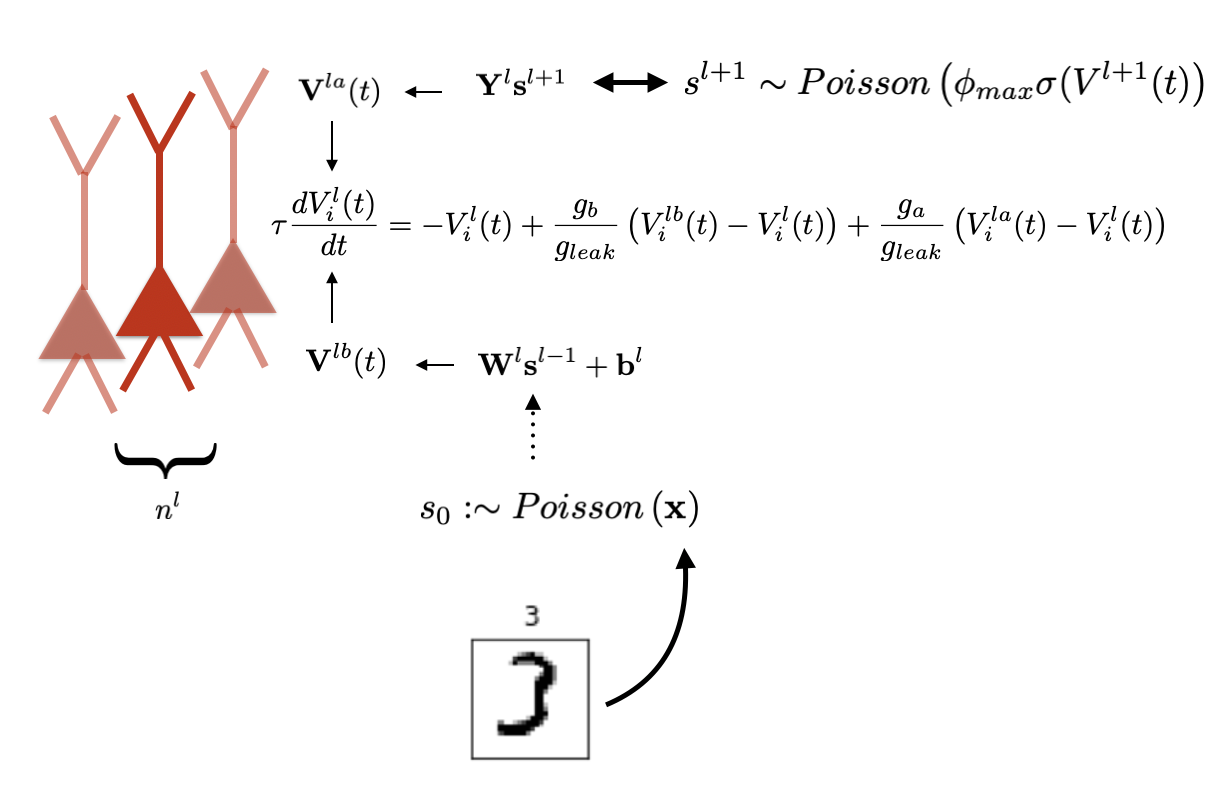
\includegraphics[width=1.05\textwidth]{../figures/report/hidden_2}
\end{frame}

%------------------------------------------------------------------------------%
\begin{frame}{\citet{guerguiev2017} - Output Layer Structure}

\centering 
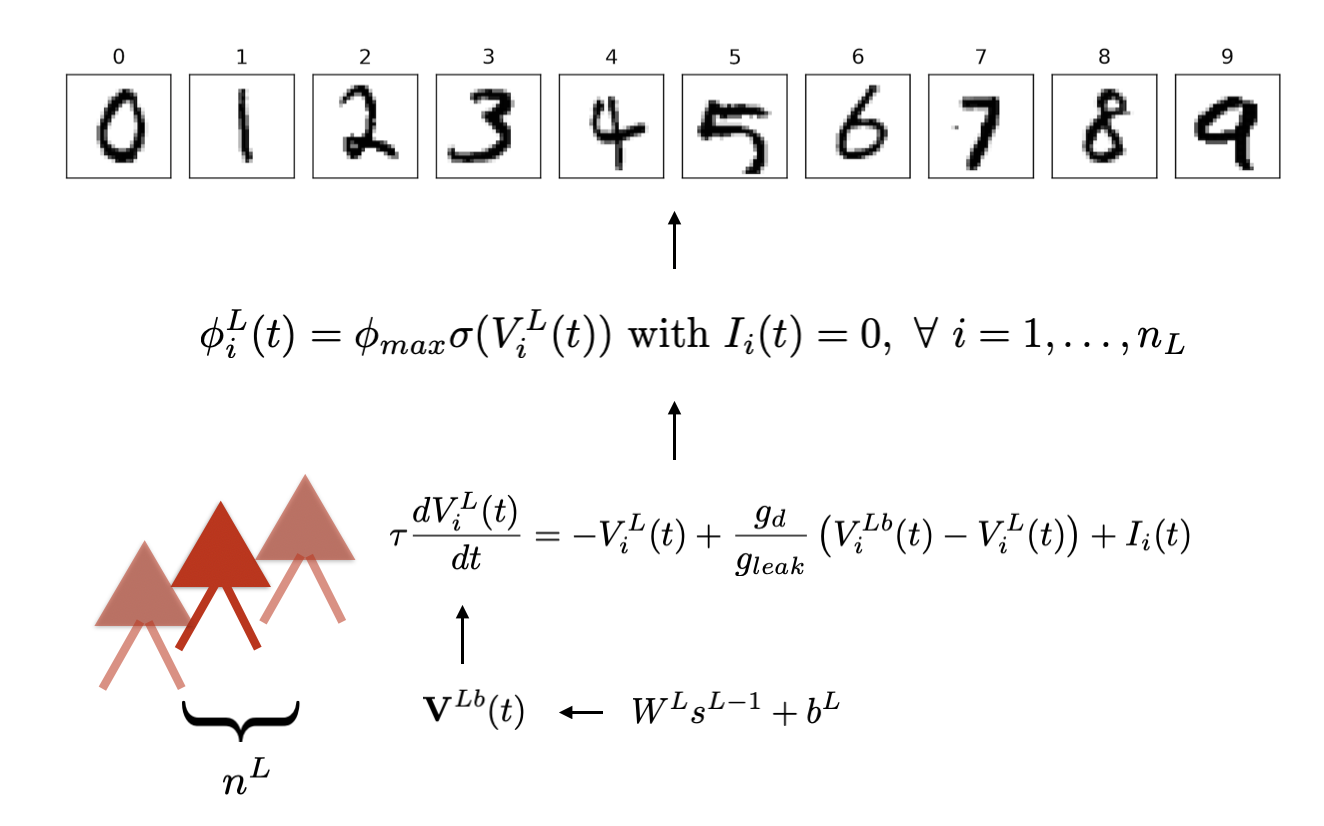
\includegraphics[width=1.05\textwidth]{../figures/report/out_1}
\end{frame}

%------------------------------------------------------------------------------%
\begin{frame}[noframenumbering]{\citet{guerguiev2017} - Output Layer Structure}

\centering 
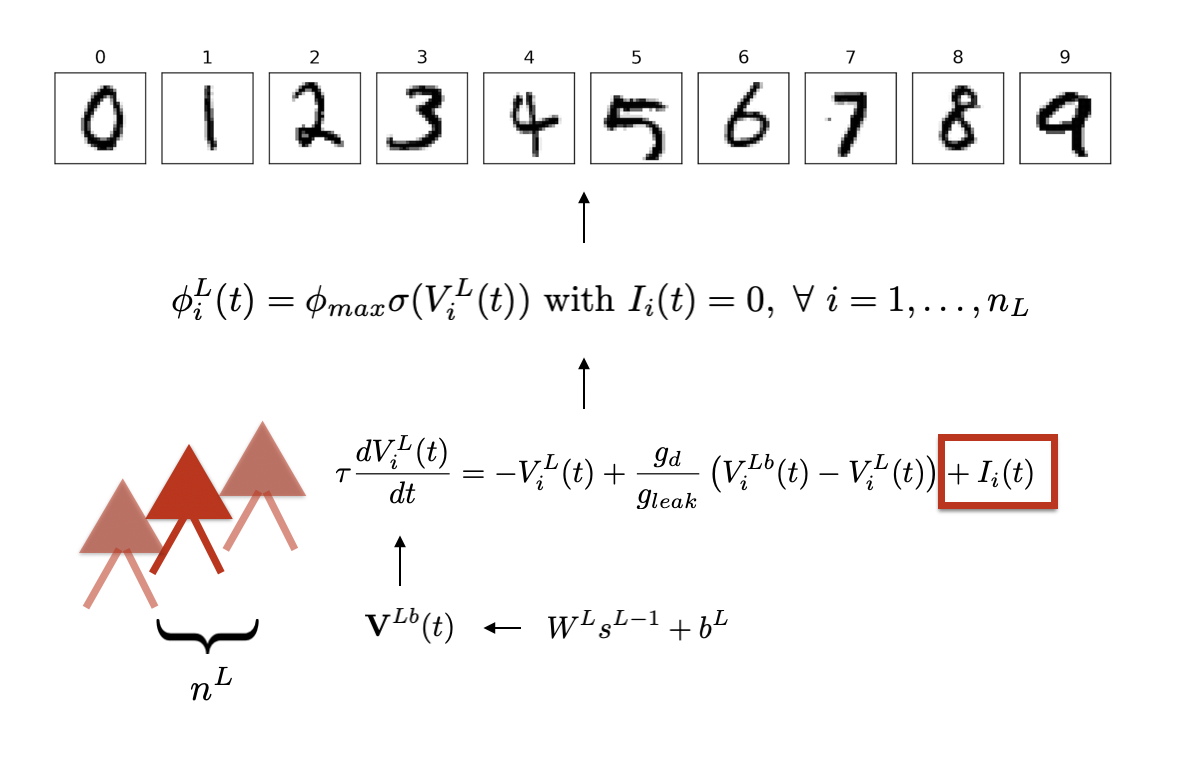
\includegraphics[width=1.1\textwidth]{../figures/report/out_2}
\end{frame}

%------------------------------------------------------------------------------%
\begin{frame}{\citet{guerguiev2017} - Credit Assignment Signals}

\centering 
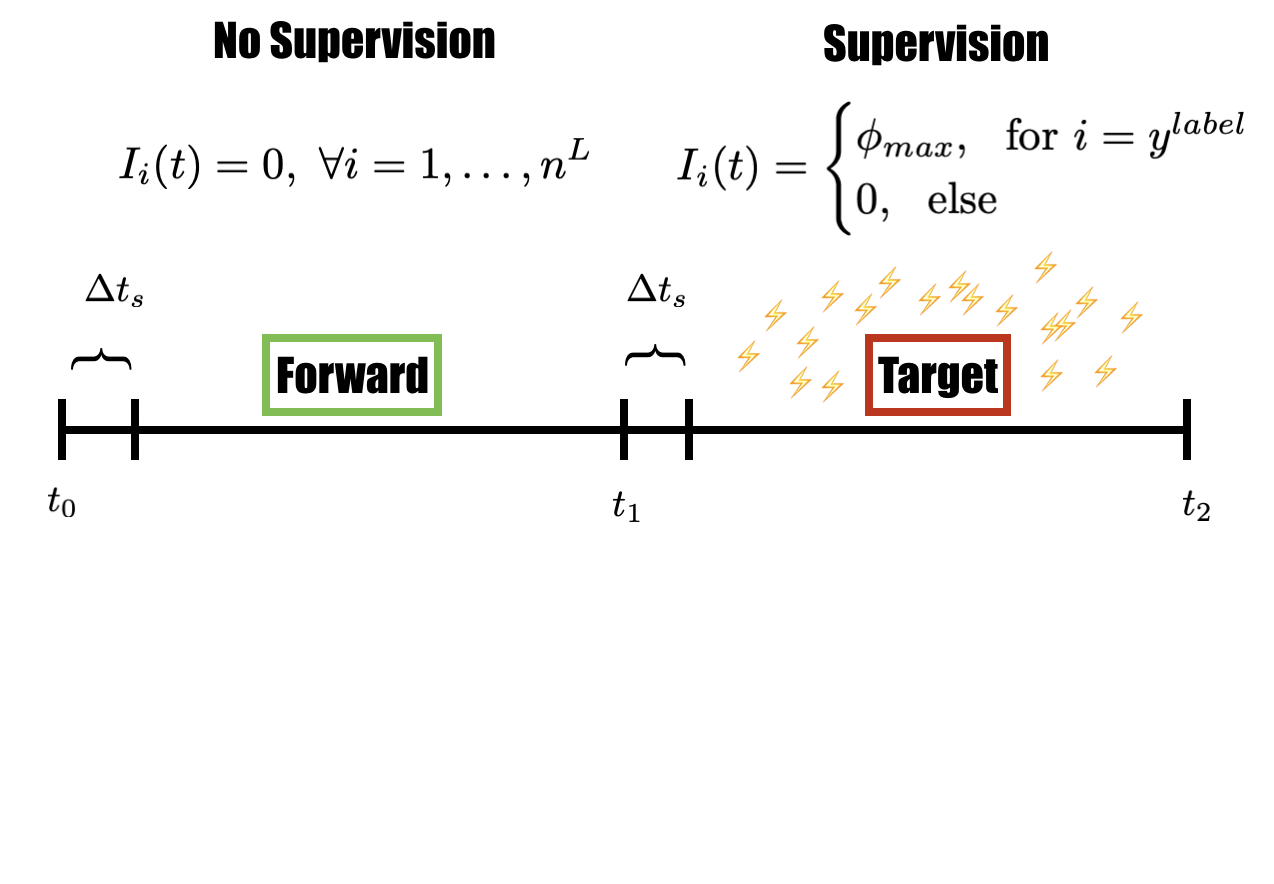
\includegraphics[width=1.05\textwidth]{../figures/report/phases_1}
         
\end{frame}
%------------------------------------------------------------------------------%
\begin{frame}[noframenumbering]{\citet{guerguiev2017} - Credit Assignment Signals}

\centering 
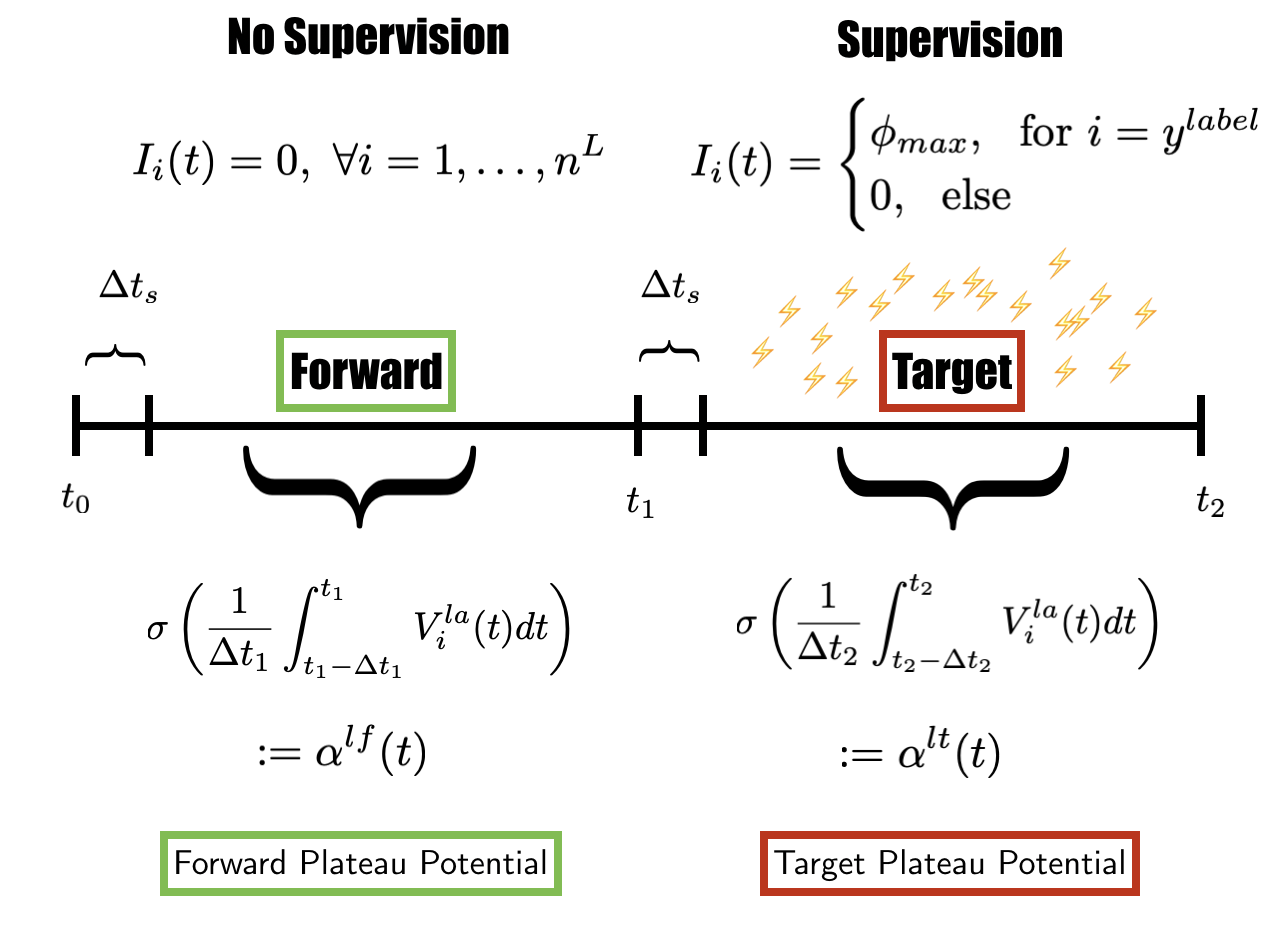
\includegraphics[width=1.05\textwidth]{../figures/report/phases_2}         

\end{frame}

%------------------------------------------------------------------------------%
\begin{frame}{\citet{guerguiev2017} - Learning}
	\vspace{0.5cm}
	\begin{tcolorbox}
	Forward phase activity $\Leftrightarrow$ Target phase activity  
	\end{tcolorbox}
	\pause

\begin{itemize}
	\item[$\Rightarrow$] Output Layer:
	\begin{itemize}
		\item[$\circ$] Target firing rates: $\phi_i^{L\star} = \frac{1}{\Delta t_2} \int_{t_1 + \Delta t_s}^{t_2} \phi_i^L(t)dt$
		\item[$\circ$] Loss function: 
	\end{itemize}
	\vspace{0.5cm}
	$$L^L = ||\phi^{L\star} - \bar{\phi}^{Lf}||_2^2 = ||\frac{1}{\Delta t_2} \int_{t_1 + \Delta t_s}^{t_2} \phi^L(t)dt - \frac{1}{\Delta t_1} \int_{t_0 + \Delta t_s}^{t_1} \phi^L(t)dt||_2^2$$
	\pause
	\item[$\Rightarrow$] Hidden Layer:
	\begin{itemize}
		\item[$\circ$] Target firing rates: $\phi_i^{l\star} = \bar{\phi}_i^{lf} + \alpha_i^{lt} - \alpha_i^{lf}$
		\item[$\circ$] Loss function:
	\end{itemize}
	\vspace{0.5cm}
	$$L^l = ||\phi^{l\star} - \bar{\phi}^{lf}||_2^2 = ||\alpha^{lt} - \alpha^{lf}||_2^2$$
	\pause
	\item[$\Rightarrow$] Local error minimization via gradient descent
\end{itemize}
\end{frame}

%------------------------------------------------------------------------------%

\begin{frame}[noframenumbering]{Empirical Investigations}
	\begin{figure}
		\centering
		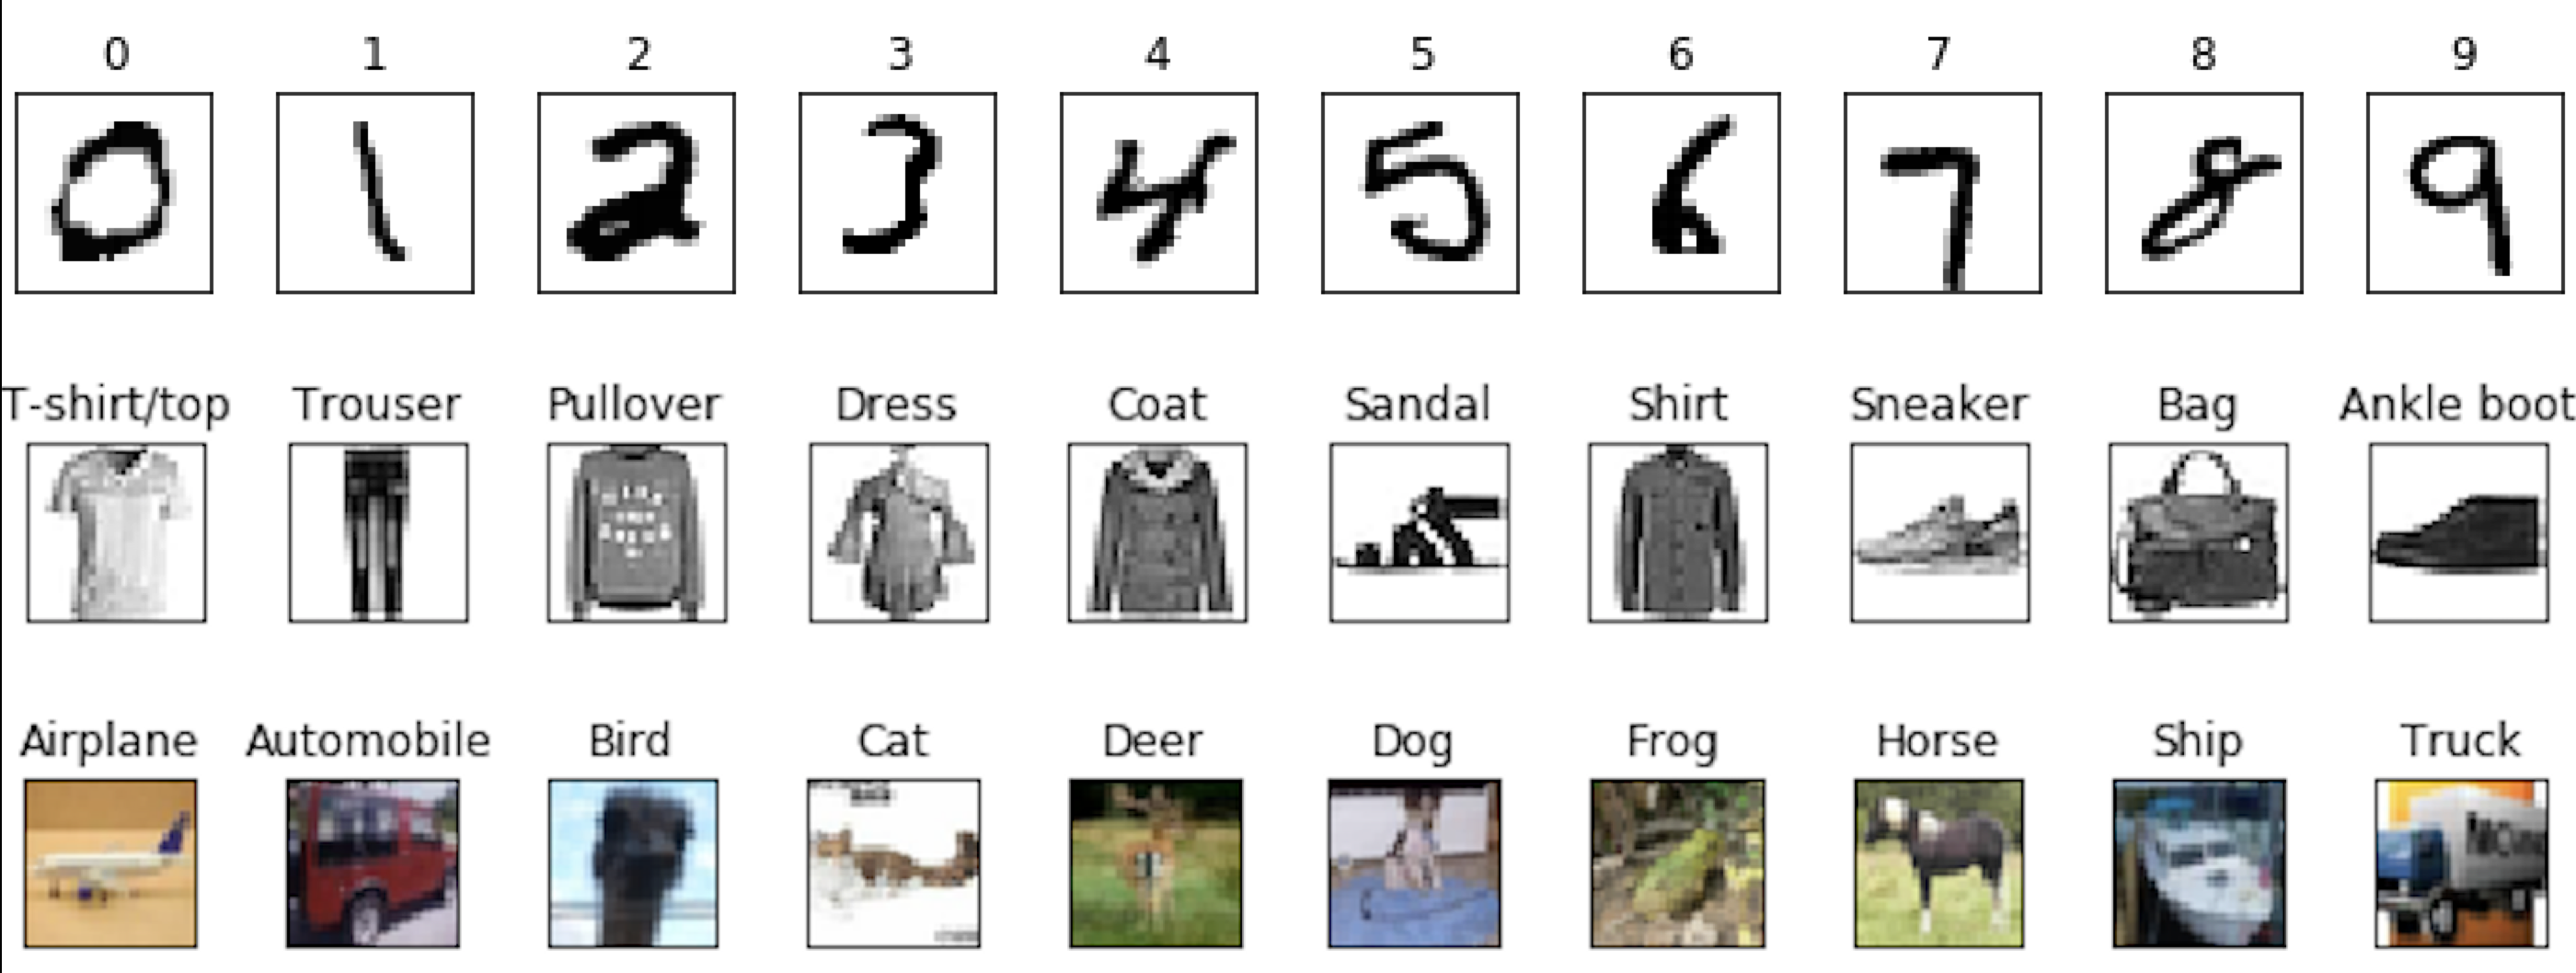
\includegraphics[width=\textwidth]{../figures/report/datasets}
	\end{figure}
\end{frame}

%------------------------------------------------------------------------------%

\begin{frame}{State-of-the-Art Performance}
	\begin{figure}
		\centering
		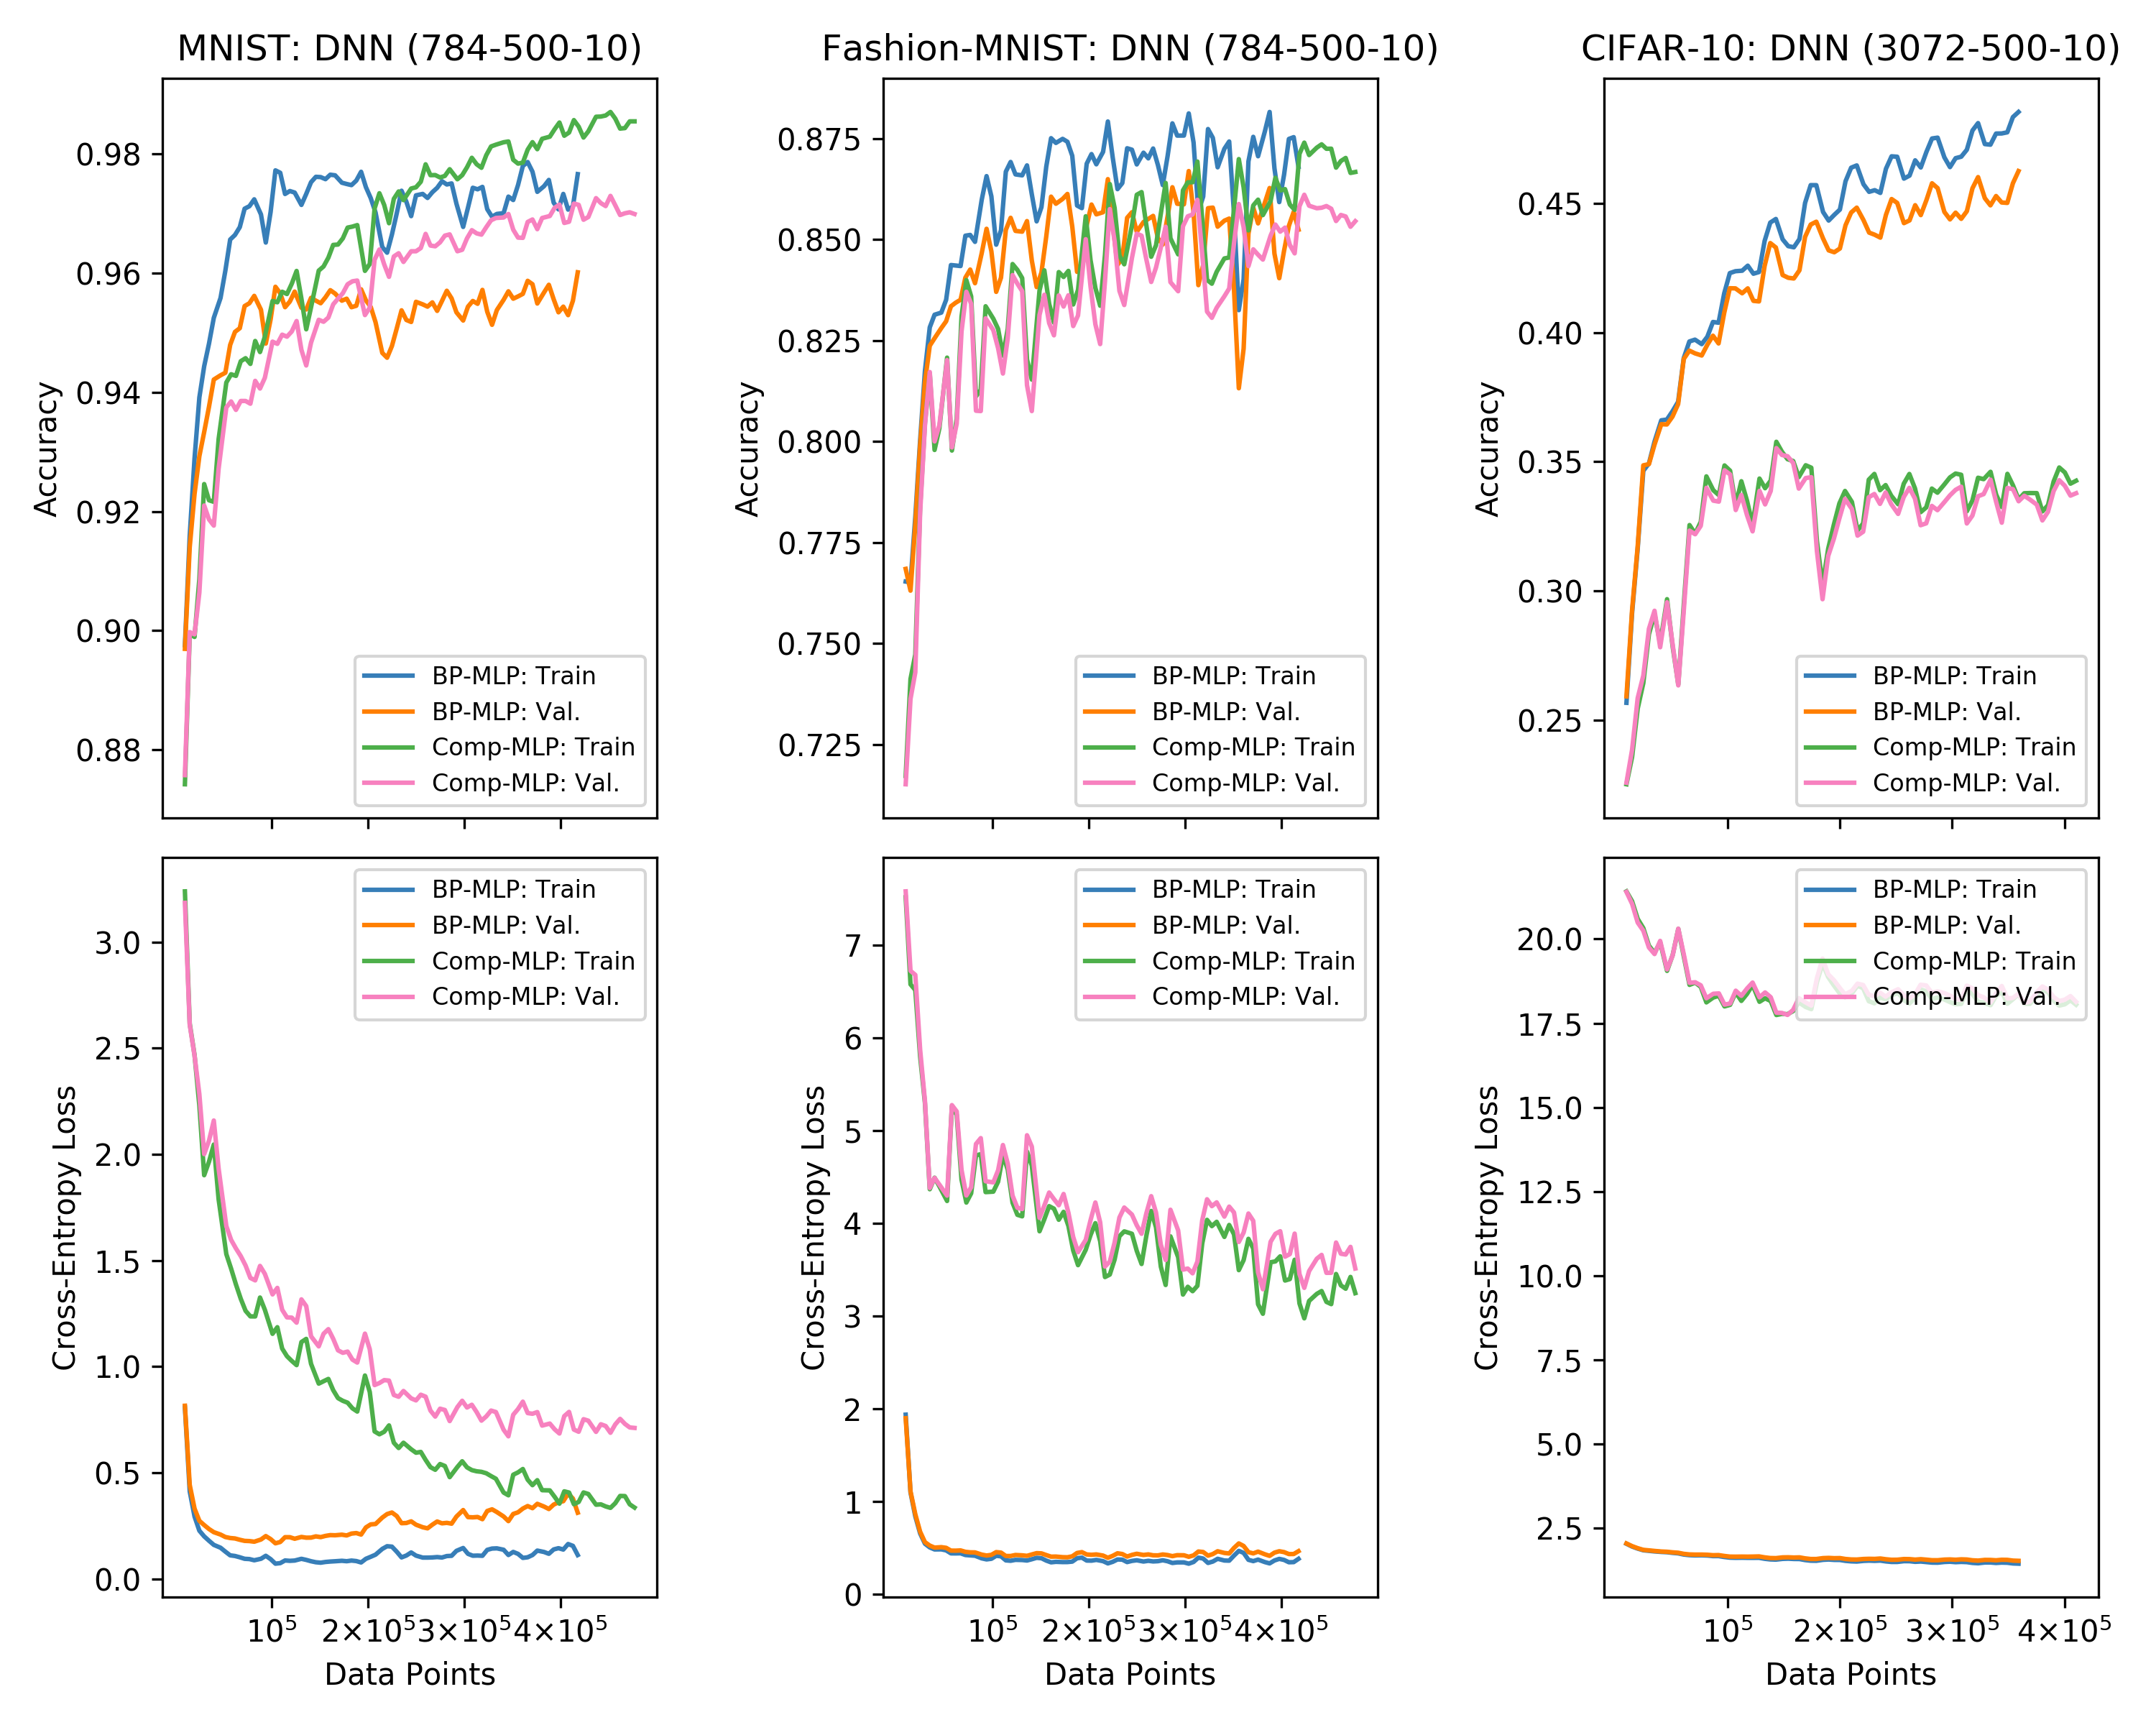
\includegraphics[width=\textwidth]{../figures/learning}
	\end{figure}
\end{frame}

%------------------------------------------------------------------------------%

\begin{frame}{Fast convergence or Overfitting?}
	\begin{figure}
		\centering
		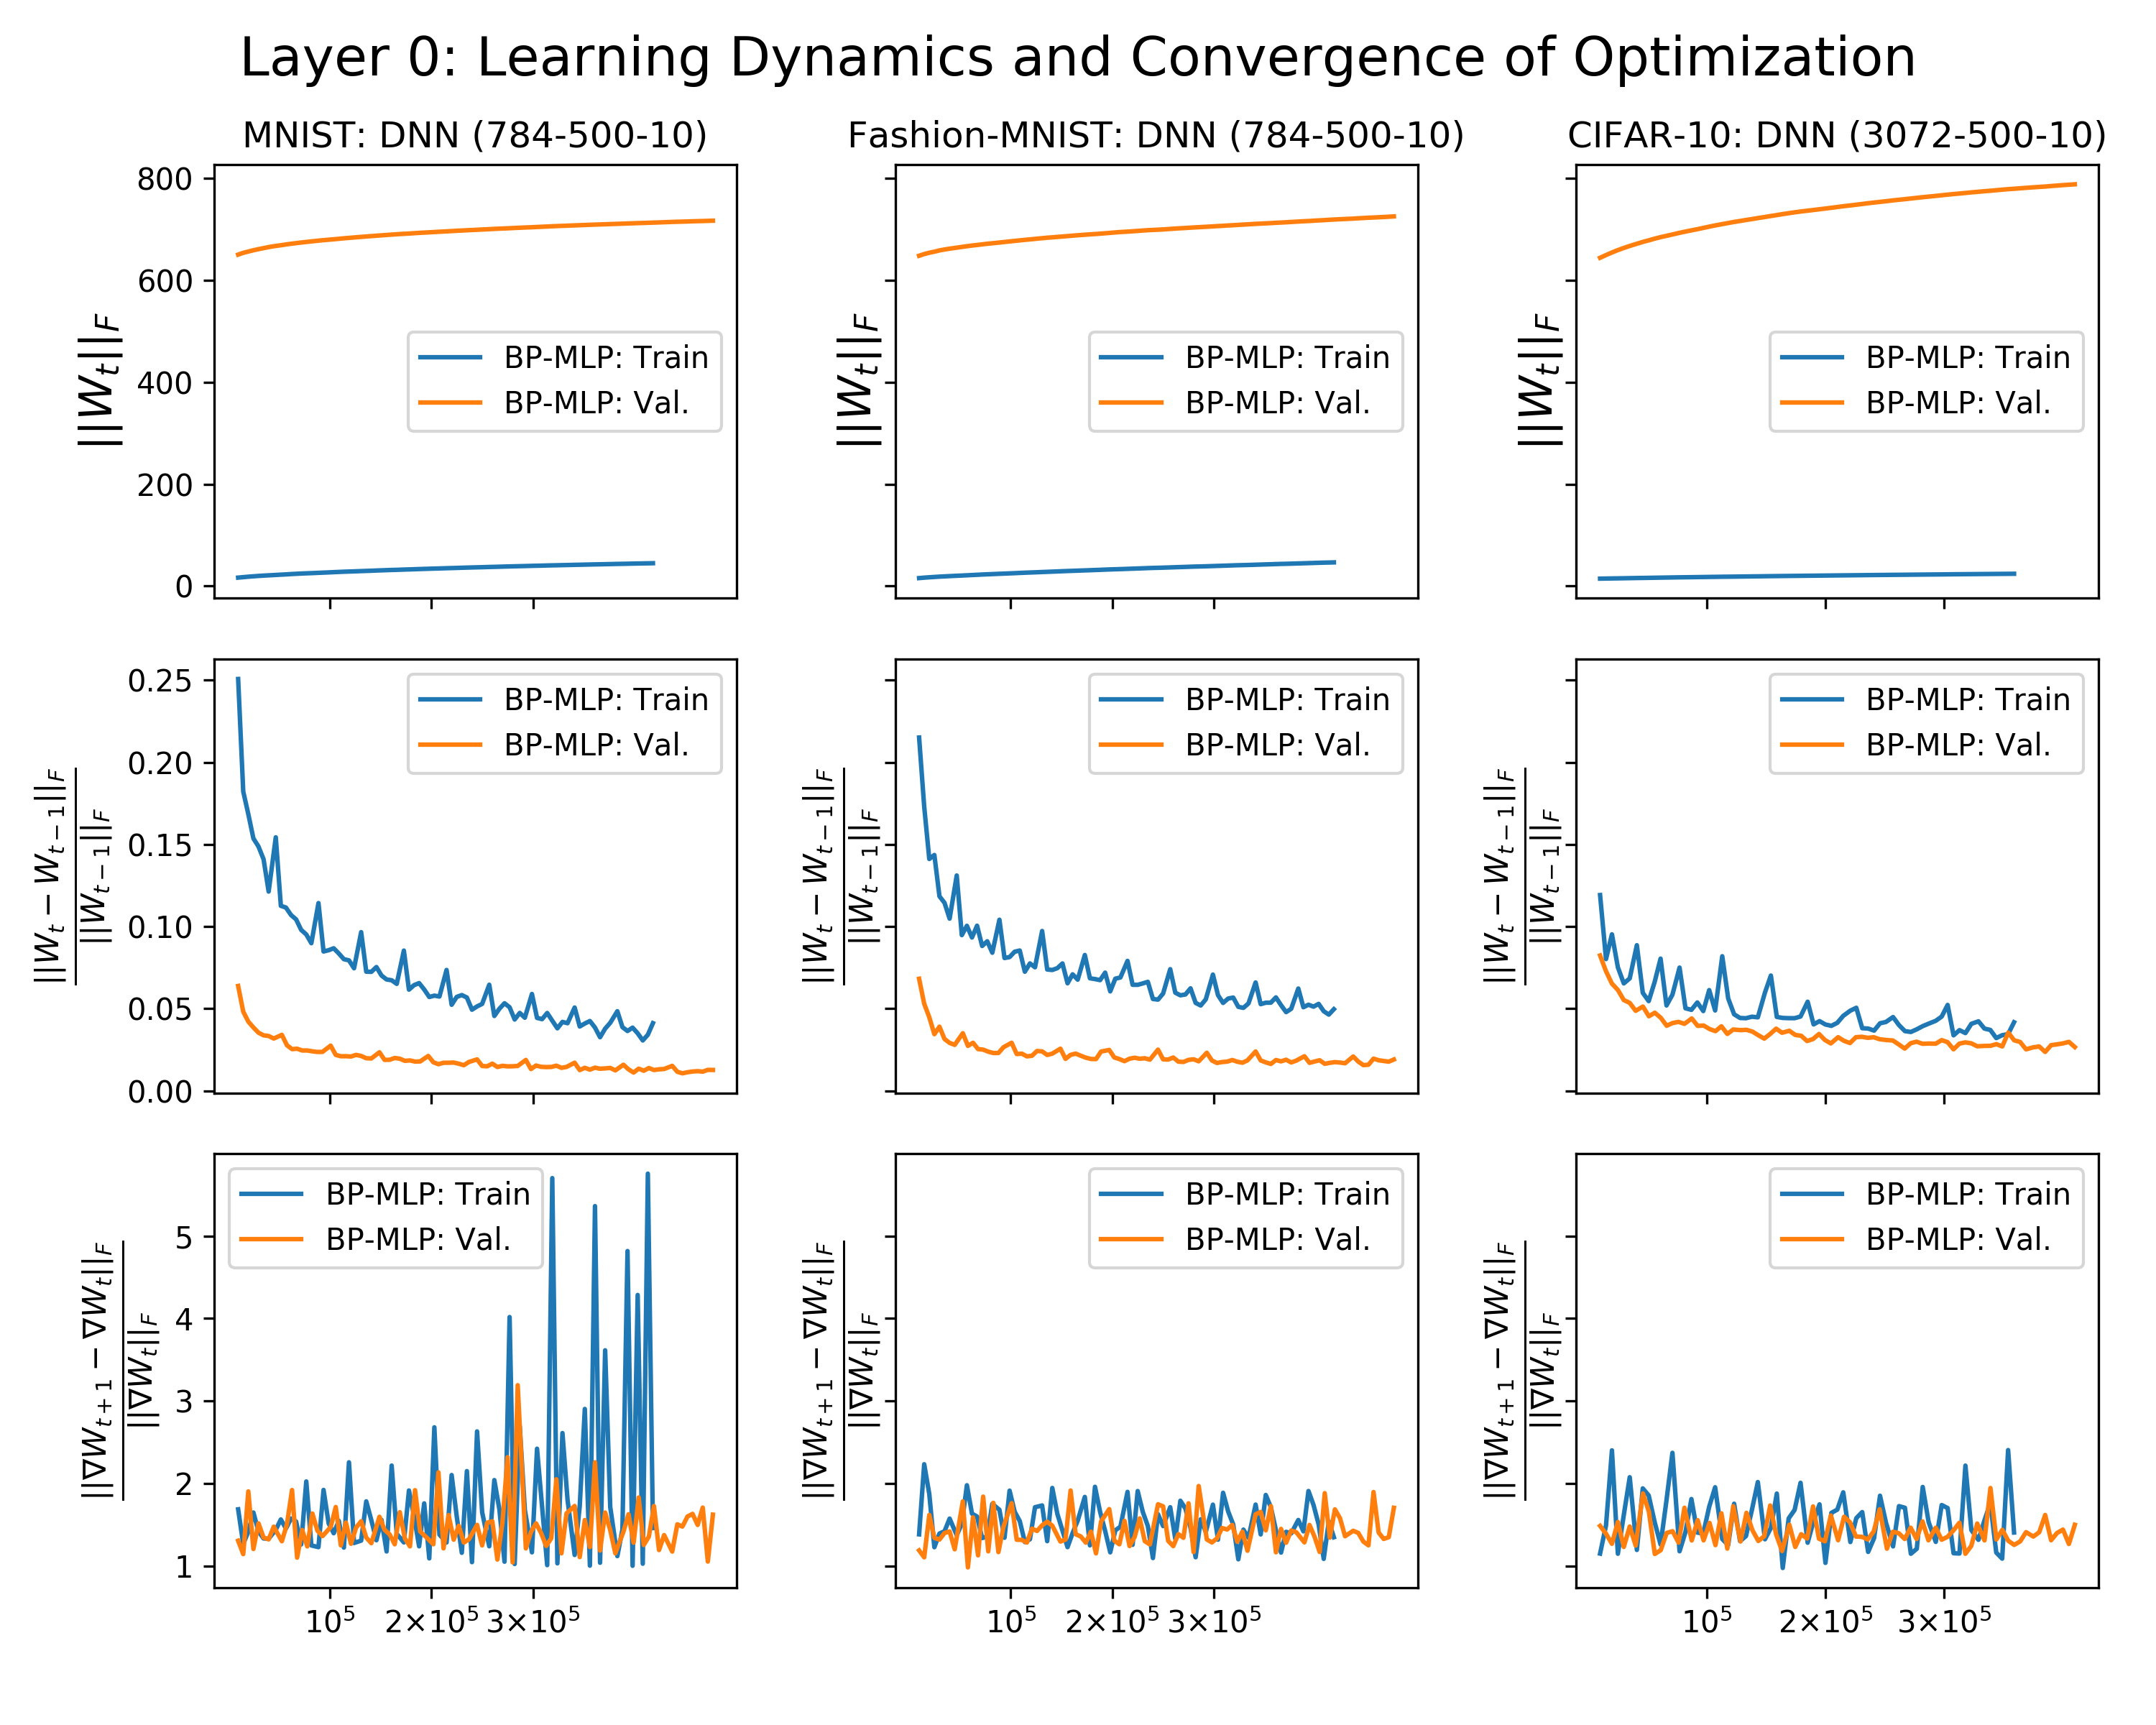
\includegraphics[width=\textwidth]{../figures/dynamics_l0}
	\end{figure}
\end{frame}

%------------------------------------------------------------------------------%

\begin{frame}{Well... Robustness?}
	\begin{figure}
		\centering
		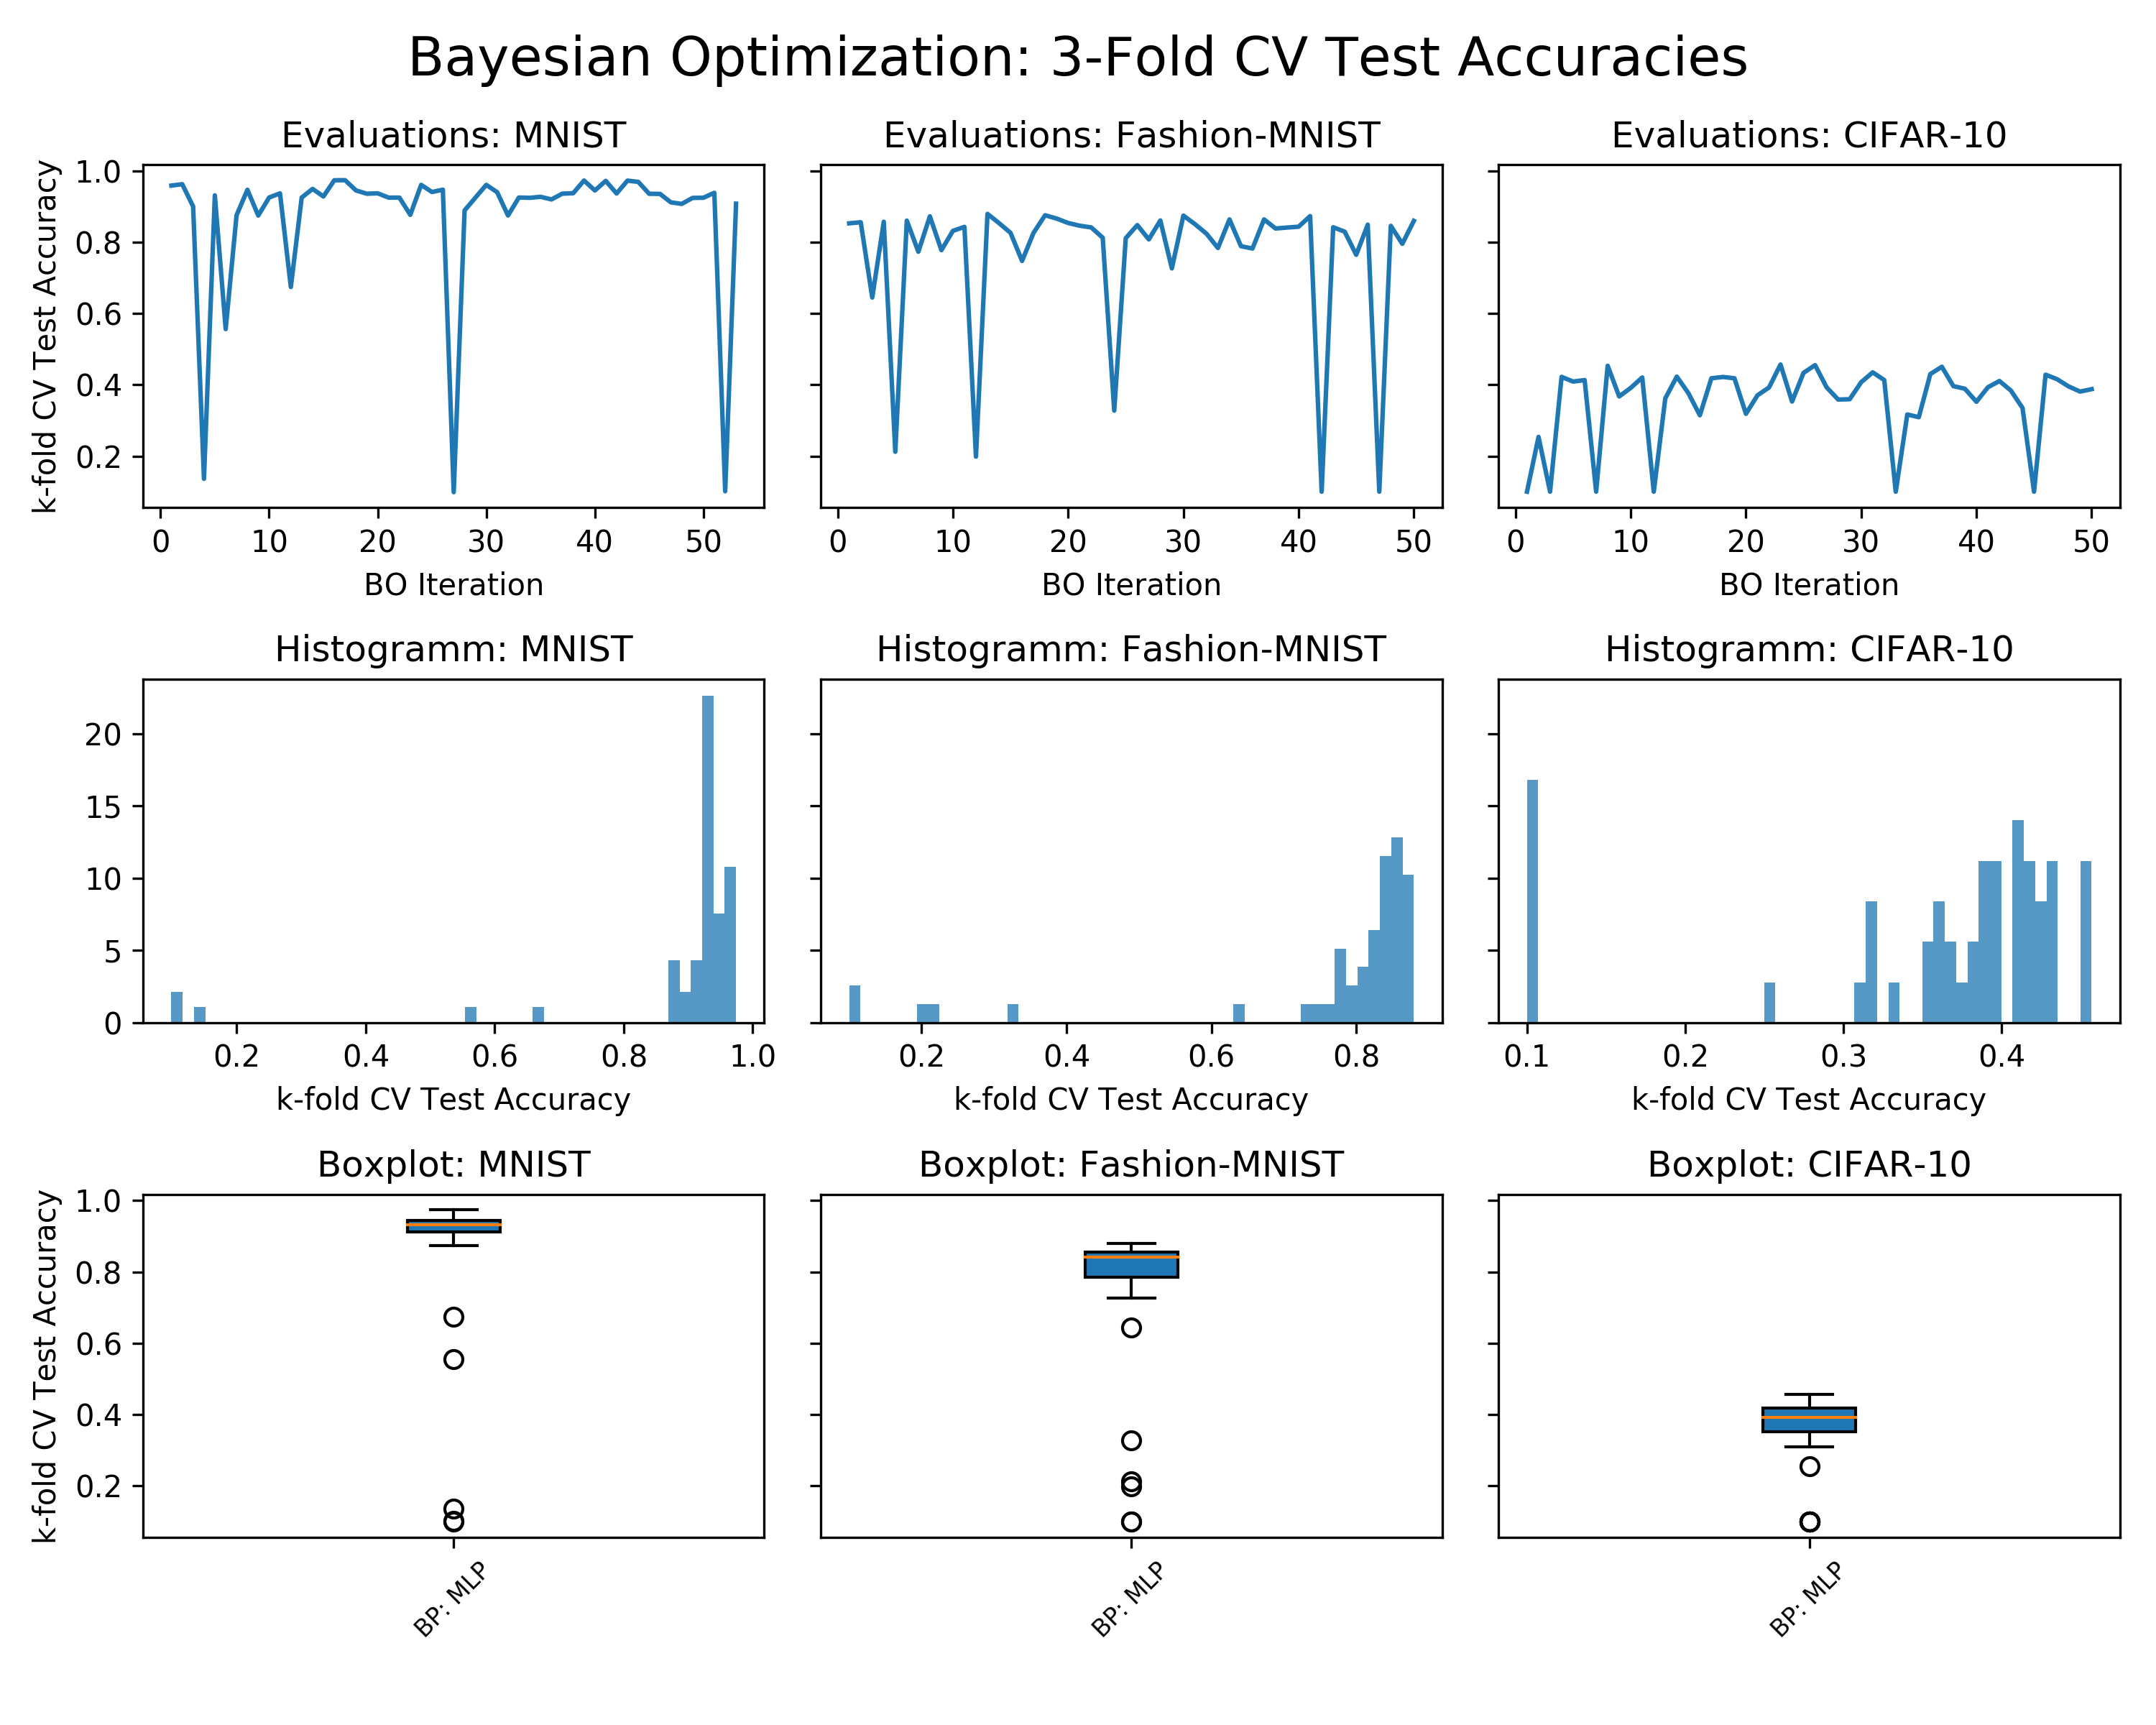
\includegraphics[width=\textwidth]{../figures/bayes_opt_comparison}
	\end{figure}
\end{frame}

%------------------------------------------------------------------------------%
\begin{frame}{\citet{guerguiev2017} - Accomplishments/Problems}

\begin{todolist}
	\item[\done] Physiological plausible electrical segregation
	\item[\done] Signal can be used to exploit depth in near-continuous time
	\item[\wontfix] \textbf{Computational} Problems
	\begin{itemize}
		\item[$\to$] Expensive/slow training
		\item[$\rightarrow$] Non-robust!
	\end{itemize}
	\item[\wontfix] \textbf{Physiological} Problems
	\begin{itemize}
	\item[$\rightarrow$] How is the teaching signal internally generated - Mismatch neurons?
	\item[$\rightarrow$] 2 global phases? - Length sampled from inverse Gaussian
	\item[$\rightarrow$] Stoch. gen. of plateau potentials - apical calcium spikes
	\end{itemize}
\end{todolist}
\end{frame}


\begin{frame}{Where to go from here?}
	\begin{tabular}{cl}
	       \begin{tabular}{l}
             \parbox{0.6\linewidth}{%  change the parbox width as appropiate
            \begin{itemize}
				\item[$\to$] \citet{sacramento2018}: Local error from mismatch with local \textbf{interneurons}
				\begin{itemize}
					\item[$\Rightarrow$] Lateral $\Leftrightarrow$ Apical
					\item[$\Rightarrow$] No separate phases
				\end{itemize}
				\item[$\to$] \citet{naud_2018}:  \textbf{Multiplexing}
				\begin{itemize}
					\item[$\Rightarrow$] Burst Fraction $\Leftrightarrow$ Apical $\Downarrow$
					\item[$\Rightarrow$] Event Rate $\Leftrightarrow$ Somatic $\Uparrow$
				\end{itemize}
            \end{itemize}
    }
         \end{tabular} 
           & \begin{tabular}{c}
           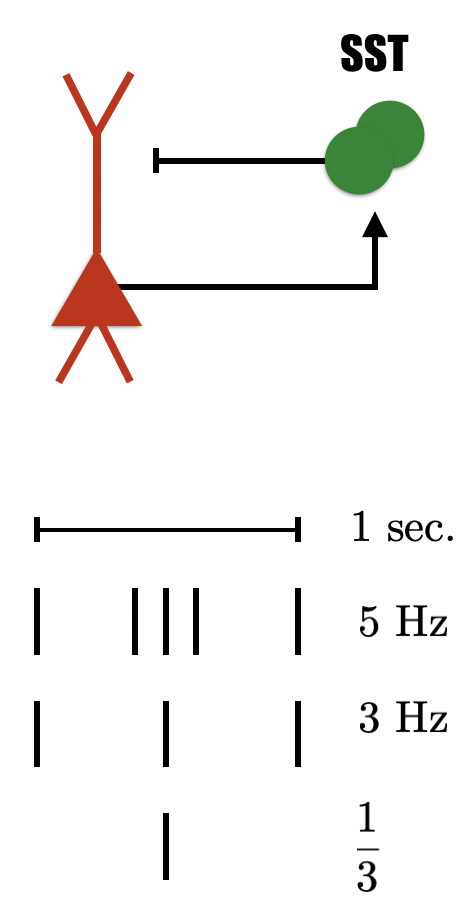
\includegraphics[width=3cm]{../figures/report/outlook}
           \end{tabular}  \\
\end{tabular}
\end{frame}


%------------------------------------------------------------------------------%

\begin{frame}[allowframebreaks, noframenumbering]{References}
   \begin{tiny}
   \setbeamertemplate{bibliography item}[text]
   \bibliographystyle{authordate1}
   \bibliography{main.bib}
   \end{tiny}
\end{frame}


%------------------------------------------------------------------------------%



\end{document} 